\documentclass[11pt]{article}
\usepackage[margin=1in]{geometry}
\usepackage{amsmath,amssymb}
\usepackage{booktabs}
\usepackage{graphicx}
\usepackage{xcolor}
\usepackage[numbers,sort&compress]{natbib}
\usepackage{hyperref}
\hypersetup{colorlinks=true,allcolors=blue!50!black}

\newcommand{\TODO}[1]{\textcolor{red}{[TODO: #1]}}
\newcommand{\RESULT}[1]{\textcolor{blue}{[#1]}}

\title{Leakage is not uniform:\\
duplicate-image leakage concentrates on the classes that matter}
\author{}
\date{}

\begin{document}
\maketitle

\begin{abstract}
That dermatology image datasets contain several photographs of the same patient or lesion,
that splitting them by image therefore leaks, and that the remedy is to split by patient or
lesion, are all \textbf{established}. HAM10000's own release paper reports its per-lesion
image counts; \citet{fitzpatrick_audit2024} document leakage in HAM10000, DermaMNIST and
Fitzpatrick17k and release corrected partitions; patient-level partitioning is standard
practice in a growing part of the literature. We do not claim otherwise and this paper is
not about rediscovering it.

We report three things that appear not to have been said. First, \textbf{the leak is not
uniform across classes, and it concentrates where it hurts}: in HAM10000 an image-level
80/20 split leaks 38.5\% of the test set overall but \textbf{68.3\% of melanomas} against
29.4\% of nevi, because melanomas were photographed more often per lesion --- and melanoma
sensitivity is the metric that benchmark is reported for. Second, \textbf{ACNE04}
\citep{wu2019}, the standard acne-severity benchmark, has to our knowledge never been
audited, and it leaks worse than either dataset where this is known: its 1{,}457
photographs are approximately 550--750 individuals, and \textbf{77.5\%} of every published
test fold shows a person who also appears in training. We measure what that is worth ---
an identical classifier gains \textbf{4.5 points of balanced accuracy} (95\% CI 2.3--7.0)
from image-level splitting, concentrated in the two rare grades ($+9.9$, $+9.0$) and absent
from the two majority grades, reproducing the same class-conditional shape by an opposite
mechanism. Third, \textbf{the instruments used to detect any of this are themselves
miscalibrated on homogeneous corpora}: the SSCD threshold behind the field's reference
memorisation rate flags 82.6\% of real ACNE04 images as copies of one another, and we give a
calibration procedure. The ACNE04 audit also turns up 38 byte-identical duplicate pairs,
eight label-conflicting, and a severity label that a second expert team's re-annotation of
the same photographs reproduces on only 30.1\% of images. Every number reproduces from
public data; the class-conditional result needs no images and no model.
\end{abstract}

\section{Introduction}

Dermatology image datasets photograph patients and lesions more than once. Splitting them
by image rather than by subject therefore puts the same lesion on both sides of the
boundary, and the field knows this: HAM10000's release paper reports that its 10{,}015
images come from 7{,}470 lesions, \citet{fitzpatrick_audit2024} document the consequence
across three datasets and publish corrected partitions, \citet{cleanpatrick2025} build a
cleaning benchmark, and a growing share of recent work partitions at the patient level as a
matter of course.

Our starting question was different --- whether generated images can substitute for real
ones in acne severity grading --- and we needed clean splits to ask it. Building them
surfaced three things the existing treatments of leakage do not cover.

\paragraph{The leak has a shape.} Leakage is reported as a single rate, and a single rate
averages over classes that are not equally affected. Duplication is a clinical decision:
worrying lesions get photographed more. In HAM10000 melanomas average 1.81 images per
lesion against 1.24 for nevi, so an image-level split leaks 68.3\% of melanoma test images
and 29.4\% of nevi. The overall figure, 38.5\%, describes neither. Because melanoma
sensitivity is what that benchmark is reported for, the aggregate rate understates the
problem exactly where it matters.

\paragraph{ACNE04 has never been audited, and it is worse.} The benchmark for automated
acne grading has no published data-quality analysis that we could find. Its subject
structure is not in any metadata --- it takes a face-recognition model to see --- and it is
severe: roughly 550--750 people across 1{,}457 photographs, with 77.5\% of every published
test fold showing someone who also appears in training. We measure the cost, which nobody
has done on a dataset where the leak is this large, and find the same class-conditional
shape arriving by the opposite mechanism.

\paragraph{The instruments need calibrating.} Every published or default similarity
threshold we reached for --- perceptual hashing, CLIP, and the SSCD threshold that
establishes the reference memorisation rate for generative models --- fails on a corpus
where all images are the same kind of picture, which is what medical imaging corpora are.

\section{Data and instruments}

We audit \texttt{Classification.tar} as distributed from the ACNE04 release
\citep{wu2019}: 1{,}457 JPEG images and ten label files giving a fixed five-fold split
(1{,}165 train / 292 test per fold). Each label row is
\texttt{<file> <grade> <lesion\_count>}.

\paragraph{The grade is derived, not annotated.}
For all 1{,}457 records the grade is exactly the Hayashi banding of the count ---
1--5 $\rightarrow$ 0, 6--20 $\rightarrow$ 1, 21--50 $\rightarrow$ 2, $>$50 $\rightarrow$
3 --- with zero exceptions. The severity label carries no information beyond the count,
so all label noise originates in counting. This makes every repeated annotation of the
same image a direct measurement of that noise.

\paragraph{Deduplication instruments must be calibrated on this corpus.}
Every ACNE04 image is a half-face shot at roughly $70^\circ$ against a dark background,
so generic perceptual and semantic embeddings have little to work with. At the common
perceptual-hash setting (Hamming $\leq 8$), linkage percolates into a single cluster
holding 14.7\% of the corpus, and the linked pairs are different people in the same
pose. CLIP ViT-B/32 fails identically: the median pairwise cosine across the whole
corpus is 0.83 and percolation begins at 0.96. We use Hamming $\leq 2$ and cosine
$\geq 0.98$, calibrated against the 38 byte-identical pairs, all of which sit at cosine
1.0000.

\paragraph{Face detection needs padding, or it silently fails.}
For the identity analysis we embed with ArcFace (InsightFace \texttt{buffalo\_l}).
Detection succeeds on \textbf{9.3\%} of ACNE04 images as distributed and \textbf{96.1\%}
after padding the border by 60\% of the long side: these are close crops in which the
face fills the frame, and the detector expects a face to occupy a fraction of the image.
We record this because a pipeline that omits the padding concludes, silently and
wrongly, that the dataset contains almost no faces.

\section{ACNE04 is about 600 people}
\label{sec:subjects}

\begin{figure}[t]
\centering
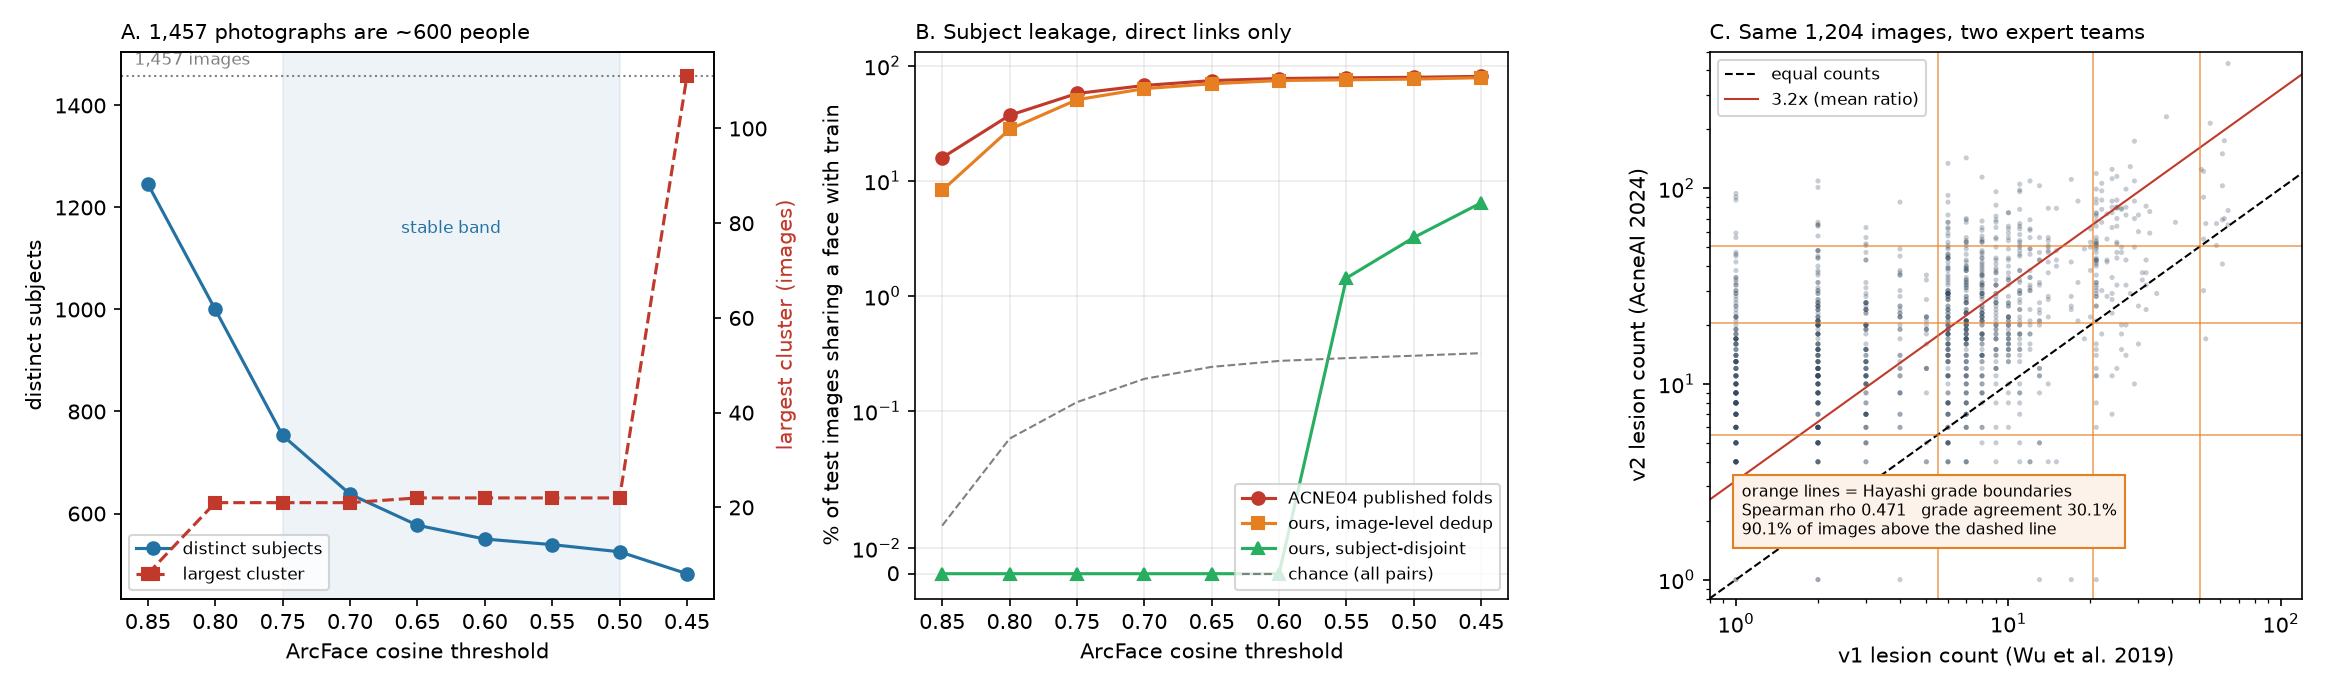
\includegraphics[width=\textwidth]{../docs/examples/acne04_leakage.png}
\caption{\textbf{A.} Union-find over ArcFace cosine: the number of distinct subjects is
stable from 0.75 down to 0.50 and percolates only at 0.45. \textbf{B.} Subject leakage,
counting only direct links (no transitive closure), against the chance rate --- the
share of all image pairs above the same threshold. The published folds and our own
image-level splits are indistinguishable and two to three orders of magnitude above
chance. \textbf{C.} Lesion counts for the 1{,}204 images annotated by both teams, log
scale, with the Hayashi grade boundaries marked.}
\label{fig:leakage}
\end{figure}

Union-find over ArcFace cosine gives 550--750 distinct individuals across the 1{,}457
photographs, with 84\% of images belonging to a subject that appears more than once and
a largest subject of 22 images. The clustering is stable across the whole band from
cosine 0.75 to 0.50 and percolates only at 0.45 (Figure~\ref{fig:leakage}A), which is
the signature of real structure rather than a threshold artefact; the 38 byte-identical
pairs sit at cosine 1.000, calibrating the instrument. Visual inspection of the largest
clusters confirms them: each is one individual photographed from several angles across
several sessions.

\paragraph{Negative control: identity, or shared capture conditions?}
The obvious objection to any embedding-based leakage claim is that the model may be
scoring the photo shoot rather than the person. On this corpus the objection has teeth:
76\% of images share one resolution, 97.8--99.7\% of linked pairs sit inside a single
resolution group against a 63.2\% chance baseline, and only 4\% of identity clusters span
more than one resolution. That pattern has a benign reading (one person, one session, one
camera) and a fatal one (the model is scoring capture conditions), and they are separable.
Restricting to the dominant resolution group --- 1{,}107 images, one camera, one setup ---
the median pairwise cosine is \textbf{0.103}, the 99th percentile is 0.342, and only
\textbf{0.423\%} of pairs clear 0.60 with \textbf{0.029\%} clearing 0.85. Had capture
conditions driven the similarity, the distribution inside that homogeneous group would be
shifted high and unimodal. It is low with a thin distinct tail, so the clusters are people
and the resolution concentration is the benign reading.

We report leakage in the most conservative form available. A test image counts as leaked
only if \emph{it is itself} above threshold to some individual training image --- no
clusters, no chaining --- and we give alongside it the chance rate, the share of all
image pairs in the corpus above that threshold, so the false-positive budget is visible
(Table~\ref{tab:subject}).

\begin{table}[t]
\centering
\begin{tabular}{lcccccc}
\toprule
cosine $\geq$ & chance rate & published folds & ours, image-level & ours, subject-disjoint \\
\midrule
0.85 & 0.019\% & \textbf{15.9\%} & 8.3\% & 0.0\% \\
0.80 & 0.058\% & 37.1\% & 28.1\% & 0.0\% \\
0.75 & 0.120\% & 57.5\% & 50.7\% & 0.0\% \\
0.70 & 0.191\% & 67.4\% & 63.3\% & 0.0\% \\
0.60 & 0.273\% & \textbf{77.5\%} & 74.5\% & 0.0\% \\
0.50 & 0.303\% & 79.4\% & 76.6\% & 3.2\% \\
\bottomrule
\end{tabular}
\caption{Share of test images sharing an identity with the training split, direct links
only. At cosine 0.85 fewer than one image pair in five thousand qualifies by chance, and
one published test image in six is a person who is also in training.}
\label{tab:subject}
\end{table}

Our own perceptually deduplicated splits leak just as badly, because deduplication and
identity grouping answer different questions. Grouping by identity as well gives 604
subjects and eliminates the leakage above the grouping threshold, with splits still
well formed (948 / 218 / 291, all classes present in all splits). The residual 3.2\% at
cosine 0.50 is reported rather than tuned away: grouping at threshold $T$ guarantees
disjointness above $T$ only.

\paragraph{Why this is worse than duplicate leakage.}
Severity is graded from lesion counts on \emph{half} the face, so two photographs of one
person from different sides legitimately carry different grades. The leakage is
therefore not label copying, which would be easy to dismiss as a rounding error. It is
that a model can learn an individual's skin, complexion, hair, background and capture
session and carry that to the test set, where the same person reappears with a different
lesion count. Published ACNE04 accuracies answer ``given other photographs of this
person, can you grade this one?'' --- not ``given a new patient, can you grade them?''
Only the second is what an acne grader is for.



\begin{figure}[t]
\centering
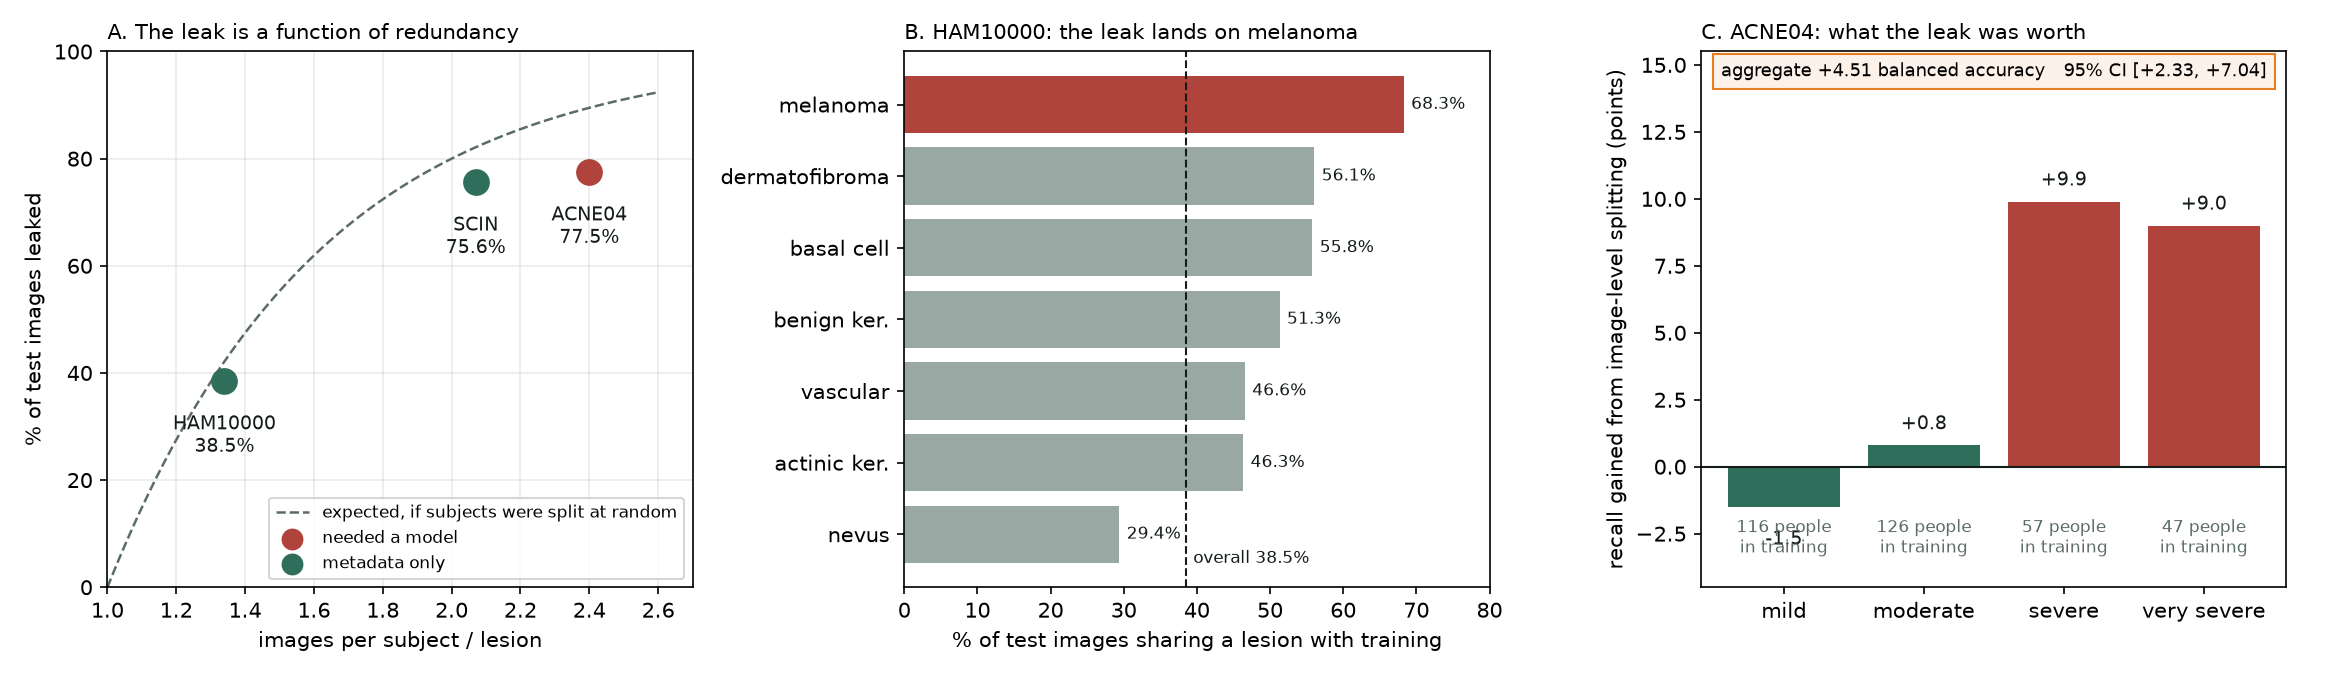
\includegraphics[width=\textwidth]{../docs/examples/three_datasets.png}
\caption{\textbf{A.} The leak is a function of redundancy: three datasets from three
institutions sit close to what a random image-level split would be expected to leak given
their images-per-subject. Two of the three measurements need only published metadata.
\textbf{B.} It does not spread evenly. HAM10000 leaks 68.3\% on melanoma against 29.4\% on
nevus, because melanomas were photographed more often per lesion --- and melanoma
sensitivity is the metric that benchmark is reported for. \textbf{C.} What it was worth on
ACNE04: recall gained from splitting by image rather than by subject, per grade, against
the number of distinct people that grade holds in training.}
\label{fig:three}
\end{figure}

\section{The same leak in a second dataset, with no model involved}
\label{sec:scin}

The strongest objection to \S\ref{sec:subjects} is that ACNE04's subject structure was
recovered with a face embedding, so the finding could be an artefact of that instrument.
SCIN removes the objection.

SCIN \citep{scin2024} --- Google Research and Stanford Medicine, 10{,}000+ crowdsourced
dermatology images --- publishes \texttt{image\_1\_path}, \texttt{image\_2\_path} and
\texttt{image\_3\_path} per case, so \texttt{case\_id} is \emph{ground truth} for ``same
subject''. No embedding, no threshold, no judgement call, and the audit is metadata-only.

\begin{table}[t]
\centering
\begin{tabular}{lcc}
\toprule
& SCIN & ACNE04 \\
\midrule
images & 10{,}407 & 1{,}457 \\
distinct subjects / cases & 5{,}033 & $\approx$550--750 \\
images per subject & 2.07 & $\approx$2.4 \\
images in a multi-image subject & 81.3\% & 84\% \\
\textbf{test images sharing a subject with training} & \textbf{75.6\%} & \textbf{77.5\%} \\
how the grouping was obtained & published metadata & ArcFace \\
\bottomrule
\end{tabular}
\caption{Two datasets from different institutions, countries, collection methods and
content, with the same structure and the same leak. SCIN's figure is what an image-level
80/20 split leaks, over 200 random splits; ACNE04's is measured on its own published folds.}
\label{tab:scin}
\end{table}

SCIN's version is arguably worse. Its multi-image cases are the \emph{same lesion} at
different distances and angles --- 2{,}289 cases carry all three of \texttt{AT\_DISTANCE},
\texttt{AT\_AN\_ANGLE} and \texttt{CLOSE\_UP} --- a tighter relationship than two
photographs of one person's two cheeks. It also carries duplication that case grouping
would not fix: 15 image files are listed under more than one \texttt{case\_id}, one of them
under eleven.

\paragraph{A third dataset, and the leak lands on melanoma.}
HAM10000 publishes \texttt{lesion\_id}, giving a third metadata-only check. Both its
duplication and the remedy are established: the release paper itself reports that 10{,}015
images come from 7{,}470 lesions with 1{,}956 lesions contributing two or more, and
\citet{fitzpatrick_audit2024} document the leakage and release corrected partitions. Our
per-lesion counts reproduce theirs exactly, which is a check on our arithmetic rather than a
finding. What appears not to have been reported is the \emph{shape} of the consequence. It leaks 38.5\% overall, about half of SCIN and ACNE04, which follows directly
from having half as many repeats per lesion (1.34 against 2.07 and $\approx$2.4).

The shape is the problem:

\begin{center}
\begin{tabular}{lrrr}
\toprule
diagnosis & images & images per lesion & test images leaked \\
\midrule
\textbf{melanoma} & 1{,}113 & \textbf{1.81} & \textbf{68.3\%} \\
basal cell carcinoma & 514 & 1.57 & 55.8\% \\
benign keratosis & 1{,}099 & 1.51 & 51.3\% \\
actinic keratosis & 327 & 1.43 & 46.3\% \\
\textbf{nevus} & 6{,}705 & \textbf{1.24} & \textbf{29.4\%} \\
\midrule
overall & 10{,}015 & 1.34 & 38.5\% \\
\bottomrule
\end{tabular}
\end{center}

Melanoma leaks at more than double the benign majority class, because melanomas were
photographed more often per lesion --- entirely reasonable clinical practice with nothing
to do with anyone's methodology. Melanoma sensitivity is \emph{the} headline metric on this
benchmark, and on an image-level split roughly two-thirds of its test images have another
photograph of the same lesion in training.

This is the same shape as \S\ref{sec:cost} found on ACNE04, reached by an opposite
mechanism: there the rare grades were photographed \emph{less}, so the clean partition was
enriched in them; here the malignant class is photographed \emph{more}, so the leaked
partition is. The general lesson is that \textbf{duplication is almost never independent of
class, so a leakage rate quoted as a single number understates its effect on the classes
anyone reports}.

\paragraph{When the leak is class-dependent, and when it is not.}
HAM10000's leak varies by a factor of 2.3 across diagnoses. Whether that is a property of
leakage or of HAM10000 is answered by SCIN, because SCIN's duplication has a different
cause. In HAM10000, how often a lesion was photographed is a \emph{clinician's decision};
in SCIN it is a \emph{fixed capture protocol} --- contributors were asked for a close-up,
one at a distance and one at an angle --- so the count reflects compliance rather than
concern. Across SCIN conditions the leak ranges 75.4--82.3\%, a spread of \textbf{6.9
points} against HAM10000's \textbf{38.9}. This makes the claim falsifiable rather than
merely observed:

\begin{quote}
Leakage is class-dependent when duplication reflects a clinical judgement, and roughly
uniform when it reflects a fixed capture protocol.
\end{quote}

ACNE04 fits the rule from the other side: there the \emph{rare} grades are photographed
\emph{less} --- 1.21 images per person at very severe against 2.30 at mild --- because
severe cases are rarer, and the leak is class-dependent in the opposite direction. In all
three the direction follows the collection process rather than anything about the images.
The practical consequence is that whether a dataset's leakage is uniform depends on
something knowable in advance, and that when the count was a clinical decision one should
expect the leak to concentrate on the class the benchmark is reported for --- because the
concern that drove the extra photograph is the same concern that drove the reporting.

\paragraph{A fourth dataset falsifies the direction.}
The rule above predicts that where duplication reflects clinical judgement, the leak
concentrates on the worrying class. ISIC 2020 --- 33{,}126 images, a clinical screening
collection carrying both \texttt{lesion\_id} and \texttt{patient\_id} --- was chosen to test
it, and fails it. At patient level the benign class leaks \textbf{99.8\%} and the malignant
class \textbf{39.3\%}: a 60-point spread, larger than HAM10000's, in the opposite direction.
Screening photographs many nevi per patient, while a malignant finding is usually one
lesion. The class dependence survives; the direction does not.

\begin{quote}
Leakage is strongly class-dependent whenever duplication is driven by a clinical process,
and \emph{the direction is not predictable from first principles} --- it depends on whether
the process re-photographs the lesion of concern or surveys the ones that are not. It has to
be measured per dataset.
\end{quote}

\paragraph{The grouping level decides whether the problem is visible at all.}
The sharper lesson is methodological. ISIC 2020 looks clean or catastrophic depending only
on which identifier the audit reaches for: 1.01 images per lesion and \textbf{2.0\%}
leakage, against 16.11 images per patient and \textbf{99.9\%}. An audit grouping by
\texttt{lesion\_id} --- the column HAM10000 taught the field to use --- would clear it.

\begin{center}
\begin{tabular}{lll}
\toprule
dataset & grouping available & where the leak is visible \\
\midrule
HAM10000 & \texttt{lesion\_id} & lesion (38.5\%) \\
ISIC 2020 & \texttt{lesion\_id}, \texttt{patient\_id} & \textbf{patient only} (99.9\% vs.\ 2.0\%) \\
SCIN & \texttt{case\_id} & case (75.6\%) \\
ACNE04 & none & requires face identity (77.5\%) \\
\bottomrule
\end{tabular}
\end{center}

Group at the coarsest level the data supports --- patient above lesion above image --- and
where no identifier exists, assume the structure is present until it has been measured.
Three of these four datasets would be misread by an audit that used the first identifier it
found.

\paragraph{A null: leakage does not vary by skin tone.}
Leakage compounding an existing fairness problem is a reasonable worry, and SCIN tests it
directly because it publishes Monk skin tone labels. Across the eight tones the leak ranges
73.2--79.8\% with no monotone trend and the extremes on the smallest strata; images per case
range 2.00--2.20. \textbf{It does not vary.} Contributors across skin tones complied with
the capture protocol equally, so the leak is distributed equally. We report this because the
opposite result would have been a significant fairness finding, and because a reader told
that leakage concentrates on clinically important classes will reasonably ask whether it
also concentrates on under-represented groups. In this dataset it does not.

\paragraph{What this changes about the claim.}
\S\ref{sec:subjects} says ACNE04's published splits leak. Together with SCIN the claim is
larger and more useful: \textbf{dermatology image datasets routinely hold several images
per subject or lesion, and image-level splitting --- the default everywhere --- leaks
between a third and three quarters of the test set in all three datasets we checked}, and
the leak concentrates on whichever class happens to have been photographed most. One
required a face-recognition model to see; two are stated in published metadata.

Three datasets are three datasets and we do not claim universality --- nor novelty for the
existence of the leak, which is established. What the comparison adds is that the rate
varies by a factor of two across datasets and tracks redundancy, and that within a dataset
it varies by a factor of two across \emph{classes} and tracks how often a clinician reached
for the camera. A benchmark's headline metric is usually reported on the class that got
photographed most. The check costs nothing: a
\texttt{groupby} where subject identifiers are published, an embedding pass where they are
not.

\section{What the leakage is worth, in points}
\label{sec:cost}

Two arms differing in exactly one thing: how the splits were drawn. The same ResNet-50,
the same ImageNet initialisation, the same hyperparameters, the same training budget and
the same five seeds. One splits at the image level after perceptual and CLIP
deduplication --- which is what every published ACNE04 result does, and what our own first
attempt did --- and carries 74.5\% subject leakage. The other groups by face identity
first and carries none. All numbers are validation; the test split has never been
unsealed.

\begin{table}[t]
\centering
\begin{tabular}{lccc}
\toprule
& image-level & subject-disjoint & difference (95\% CI) \\
\midrule
\textbf{balanced accuracy} & 0.7920 $\pm$ 0.017 & 0.7469 $\pm$ 0.016 &
  \textbf{+4.51} \; [+2.33, +7.04] \\
macro F1 & 0.7515 $\pm$ 0.025 & 0.6945 $\pm$ 0.027 & +5.69 \; [+2.37, +9.57] \\
quadratic weighted $\kappa$ & 0.8487 $\pm$ 0.016 & 0.8221 $\pm$ 0.018 &
  +2.66 \; [+0.46, +5.15] \\
plain accuracy & 0.7644 $\pm$ 0.018 & 0.7394 $\pm$ 0.025 & +2.49 \; [$-$0.80, +5.79] \\
mean absolute error & 0.2511 $\pm$ 0.024 & 0.2817 $\pm$ 0.030 & $-$3.05 \; [$-$7.63, +0.52] \\
\bottomrule
\end{tabular}
\caption{Paired by seed; bootstrap intervals over the paired differences. Splitting a
face dataset at the image level is worth about 4.5 points of balanced accuracy --- more
than the entire spread between the published methods competing on this benchmark.}
\label{tab:cost}
\end{table}

\paragraph{The bonus is not spread evenly, and where it lands is the argument.}

\begin{center}
\begin{tabular}{lcccc}
\toprule
grade & people in training & image-level & subject-disjoint & difference \\
\midrule
mild & 116 & 0.885 & 0.900 & $-$1.5 \\
moderate & 126 & 0.657 & 0.649 & +0.8 \\
severe & \textbf{57} & 0.637 & 0.538 & \textbf{+9.9} \\
very severe & \textbf{47} & 0.990 & 0.900 & \textbf{+9.0} \\
\bottomrule
\end{tabular}
\end{center}

The bonus is essentially zero on the two majority grades and about ten points on the two
rare ones --- exactly the grades with the fewest distinct subjects to memorise, which is
what the mechanism predicts: recognising an individual is worth far more when the class
holds 47 people than when it holds 126.

This also explains the aggregate row. Plain accuracy is dominated by the majority classes,
where there is no bonus, so its interval spans zero, while balanced accuracy and macro F1
weight the tail equally and show the effect clearly. \textbf{A benchmark reported in plain
accuracy will not show this leak even though it is there} --- and ACNE04 is reported in
plain accuracy.

\paragraph{The confound, and why the pattern survives it.}
The two arms have different test sets, so this comparison mixes the leakage bonus with
whatever intrinsic difficulty difference exists between them. We flag it rather than hide
it, and report alongside it a within-model analysis --- one model, one test set,
partitioned by whether the person in each test image also appears in that model's training
split (\S\ref{sec:cost}). But the per-class pattern is already difficult to explain as a
test-set artefact: a difficulty difference between two random subject-disjoint splits has
no reason to land specifically on severe and very severe while being zero on mild and
moderate. A confound would have to reproduce, by coincidence, exactly the shape the
mechanism singles out in advance.

\paragraph{The within-model contrast carries the opposite confound.}
The obvious remedy for the differing test sets is to stay inside one model and one test
set, partitioning the test images by whether the person in them also appears in training.
At cosine 0.60 that gives $+14.4$ balanced-accuracy points, consistent across seeds with
tight intervals --- roughly three times the cross-arm estimate. The disagreement is the
finding. Severity is inversely related to how many times a subject was photographed (2.30
images per person at mild, 1.21 at very severe), so a subject photographed once cannot
have a twin in training and rare-grade images leak far less. The clean partition is
43.3\% severe-or-worse against the leaked partition's 11.2\% --- a four-fold enrichment in
the hard classes. A leaked-versus-clean split is also a severity split.

Holding class fixed, which is the only comparison that partition permits, gives $+0.0$ on
mild, $+13.5$ on moderate, and $+41.8$ on severe at 13 images against 14 --- the same
ordering the cross-arm comparison found, reached by a different route with a different
bias, and the severe figure is deliberately left unquantified because 13 against 14 is not
a measurement. We report the cross-arm $+4.5$ as the headline because its confound has no
reason to align with class, whereas this one provably does.

\paragraph{What this does not say.}
It is not a claim that published ACNE04 results are overstated by 4.5 points. Those use
plain accuracy on the dataset's own folds rather than balanced accuracy on ours, and carry
77.5\% leakage against our arm's 74.5\% --- close, but not the same experiment. The
defensible statement is narrower and still substantial: on this dataset, with this
architecture and budget, image-level splitting is worth $+4.5$ balanced-accuracy points,
concentrated almost entirely in the two clinically important grades.

\section{A smaller, different leak in the same dataset}
\label{sec:duplicates}

Everything so far concerns \emph{subjects}. ACNE04 also leaks at the level of the file, in
a way that needs no model and no threshold at all, and the remaining sections report what
else the exhaustive audit of this dataset turned up.

Grouping all 1{,}457 files by MD5 of the file bytes yields 38 groups of size two: 76
files, 5.2\% of the corpus, are byte-identical copies under two filenames, usually under
two different \texttt{levleN} prefixes. Decoding to pixels and re-hashing recovers
exactly the same 38 groups.

Intersecting those groups against the dataset's own folds, \emph{every fold leaks}
(Table~\ref{tab:folds}). On average 4.25\% of each 292-image test split is byte-identical
to an image in the corresponding training split: 3.56\% where the two labels agree,
which a memorising model receives as free correct answers, and 0.68\% where they
conflict, which it cannot get right. Across all five folds, 62 distinct test images have
a byte-identical twin in training.

\begin{table}[t]
\centering
\begin{tabular}{lccccc c}
\toprule
& fold 0 & 1 & 2 & 3 & 4 & mean \\
\midrule
leaked test images & 12 & 15 & 12 & 11 & 12 & \\
as \% of the 292-image test split & 4.1 & 5.1 & 4.1 & 3.8 & 4.1 & \textbf{4.25} \\
\quad labels agree (free correct) & 2.4 & 5.1 & 3.4 & 3.8 & 3.1 & 3.56 \\
\quad labels conflict (forced error) & 1.7 & 0.0 & 0.7 & 0.0 & 1.0 & 0.68 \\
\bottomrule
\end{tabular}
\caption{Byte-identical duplicate leakage in ACNE04's published five-fold splits.}
\label{tab:folds}
\end{table}

Separately, 42 of 1{,}457 files carry a \texttt{levleN} filename prefix that disagrees
with their labelled grade, so deriving labels from filenames --- the obvious shortcut
given the naming scheme --- corrupts 2.9\% of the dataset.

\section{The label is a property of the annotation team}

\subsection{Within the release}
The 38 byte-identical pairs were annotated twice without the annotators knowing they
were the same photograph. Exact lesion-count agreement is 12/38 (31.6\%), the median
absolute count difference is 1 and the maximum is 16, and grade agreement is
\textbf{30/38 (78.9\%)}, 95\% Wilson interval 63.7--88.9\%. All eight grade
disagreements are cases where the two counts fall in different Hayashi bands; four
straddle 5/6 and four straddle 20/21. The latter are not boundary jitter but differences
of a factor of 2.4--3, and their filenames form consecutive runs, the signature of a
block ingested and counted twice by different procedures.

Reported accuracies on this benchmark sit at or above the dataset's own reproducibility
on images it annotated twice. With $n = 38$ the interval is wide and duplicates need not
be a random sample, so the defensible reading is not that published results are wrong
but that \emph{this benchmark cannot presently resolve differences of a few points}.

\subsection{Between teams}
A far better powered measurement is available. \citet{acneai2024} independently
re-annotated 1{,}204 of the same photographs, releasing 32{,}443 lesion annotations
against the original's 18{,}983 and preserving the original filenames. They count
$3.2\times$ more lesions (mean 26.9 vs.\ 8.4 per image, more on 90.1\% of shared
images), and the share of images ACNE04's labelling function would grade severe or worse
moves from 11.7\% to 46.4\%. Pearson $r$ is 0.550 and Spearman $\rho$ is 0.471.

Part of this is definitional and entirely legitimate. Hayashi's bands are defined over
\emph{inflammatory} eruptions --- papules plus pustules --- and \citet{hayashi2008}
report explicitly that global severity did not correlate with comedone counts.
\citet{acneai2024} annotate ``all lesions, either acne or non-acne lesions that look like
acne,'' including the tiny ones. \textbf{The problem is not that the teams disagree; it
is that ACNE04 publishes a count and a grade without stating which lesions were counted},
so the label depends on a convention the release never specifies.

The definitional account does not survive contact with the data. A constant change of
lesion definition would give a roughly constant ratio and preserve rank order. Instead
the per-image ratio has an interquartile range of 2.00--6.64 and a
10th-to-90th-percentile span of $11.5\times$, it falls monotonically with severity
(median $8.00\times$ where v1 counted 1--2 lesions, $2.00\times$ at 11--64), and on
8.3\% of images the second team counted \emph{fewer}. Granting the second annotation an
arbitrary monotone recalibration --- re-banding its counts by quantile matching so its
grade histogram equals the original's by construction, which removes the definitional
component entirely --- leaves:

\begin{center}
\begin{tabular}{lcc}
\toprule
& grade agreement & quadratic weighted $\kappa$ \\
\midrule
v2 counts under ACNE04's own Hayashi banding & 30.1\% & 0.296 \\
v2 counts after optimal monotone rescaling & \textbf{58.2\%} & \textbf{0.480} \\
\bottomrule
\end{tabular}
\end{center}

38.5\% of images then differ by one grade and 3.2\% by two or more, and $\rho$ does not
recover on the images with the most lesions, where relative counting noise should be
smallest ($\rho = 0.376$ for v1 count $\geq 5$, $0.297$ for $\geq 20$).

We are explicit that applying Hayashi bands to the second team's counts is \emph{our}
construction, not theirs --- they use a continuous 0--100 severity score and report
ICC 0.8 for their own method --- and that it is clinically incorrect on its face
precisely because their counts include comedones. That is the demonstration rather than
a flaw in it. It does not require deciding which team is right: two expert annotations of
the same 1{,}204 photographs do not induce the same severity ordering, and ACNE04 gives
no basis for preferring one.

\section{The instruments need calibrating too}
\label{sec:calibration}

Three times in this audit a published or library default threshold turned out to be wrong
for ACNE04, in the same way each time. The pattern is not about acne and we state it
generally, because it applies to any dataset audit that groups or flags by embedding
similarity, and medical imaging corpora are exactly where it bites --- they are
homogeneous by construction.

\begin{center}
\begin{tabular}{llr}
\toprule
instrument & usual threshold & what it does on ACNE04 \\
\midrule
perceptual hash & Hamming $\leq 8$ & one cluster holding 14.7\% of the corpus \\
CLIP ViT-B/32 & cosine $\geq 0.95$ & percolates at 0.96; corpus median cosine is 0.83 \\
SSCD \citep{somepalli2023} & $\geq 0.5$ & flags 82.6\% of real images as copies \\
\bottomrule
\end{tabular}
\end{center}

Each of those thresholds was chosen on a heterogeneous corpus --- web images, ImageNet,
LAION --- where two arbitrary items share almost nothing. Every ACNE04 image is a half-face
photograph at roughly $70^\circ$ under similar lighting, so the \emph{null} distribution of
similarity between unrelated items sits far to the right and an absolute threshold carried
across corpora measures a different thing on each.

\paragraph{Calibrating to a stated error rate.}
The remedy is to take the threshold from the corpus's own null --- the similarity between
an item and an unrelated item of the same kind --- at a stated false-positive rate. On
ACNE04, holding the per-image rate at 1\% requires \textbf{0.824} against the published
0.5. We report the null's shape alongside every rate, because a rate quoted without the
null it was measured against is not interpretable.

Two details decide whether this works, and we got both wrong before getting them right.

\emph{Per item or per pair.} Counting per pair reads reassuringly small on any large
corpus: 5.3\% of ACNE04 pairs exceed SSCD 0.5, which sounds tolerable until one notices it
means 82.6\% of \emph{images} have a false match. Per-item is the right denominator when
each item is asked an independent question, as in memorisation. It is the wrong one when
most items are \emph{expected} to have a true match --- for identity grouping, 84\% of
ACNE04 images genuinely belong to a multi-image subject, so the per-item maximum measures
the true positive and the calibration returns a threshold of 1.0.

\emph{An error rate alone is not sufficient for grouping.} Grouping takes the transitive
closure of the links, so individually rare false links chain. A 1\% per-pair rate on ACNE04
permits an identity threshold of 0.318, which merges 89.5\% of the corpus into one cluster.
Both constraints have to bind. Applied to the identity embedder, the procedure recommends a
minimum of 0.458; the 0.60 we chose by stability sweep and visual inspection sits above it
with a four-fold margin on the error budget.

\paragraph{Why this is not a footnote.}
An audit that inherits an absolute similarity threshold from web-scale copy-detection work
and applies it to a medical or face corpus reports a number dominated by its false-positive
rate. On ACNE04 the error is not marginal: 82.6\% against a true duplicate rate of 5.2\%.

It cuts both ways, and the direction matters for how such results should be read. A naive
audit of our own closed-set generator reports \textbf{12.00\%} of generated images as
near-copies of a training image at the published threshold. Calibrated on the corpus, the
figure is \textbf{0.00\%}, and the maximum similarity between any generated image and any
training image is 0.584 --- against 0.976 between two genuinely distinct real photographs.
The uncalibrated number would have condemned a generator that memorised nothing.

The same argument applies to the acne prior of \S\ref{sec:audit}, whose stated motivation
is anonymity and which reports no nearest-neighbour audit at all: on this corpus, that
claim cannot be checked with an off-the-shelf threshold either.

\section{Limitations}

The within-release reproducibility estimate rests on $n=38$ duplicate pairs, and those
pairs need not be a random sample of the corpus. The calibration procedure of
\S\ref{sec:calibration} assumes the corpus's own null is a good proxy for the null the
audit cares about; where a genuinely related pair sits inside the reference set it must be
excluded by hand, and failing to do so returns a threshold of 1.0 rather than an obviously
wrong answer. The cross-team comparison cannot
separate ``team A missed lesions'' from ``team B over-segmented'' without a third
annotation; our claim is symmetric and does not require assigning fault. Identity
clustering rests on an ArcFace threshold; we report the full threshold sweep and the
chance rate rather than a single operating point, and the most conservative figure
(15.9\% at cosine 0.85) is the one we would defend. 57 of 1{,}457 images yield no face
embedding and are excluded from the identity analysis.

\section{Reproducibility}

All findings reproduce from the public archive and the public v2 annotations:

\begin{verbatim}
python scripts/audit_acne04.py                  # duplicates, fold leakage, noise
python scripts/audit_acne04_subjects.py         # identity structure and leakage
python scripts/compare_acne04_versions.py --v2 <acne04v2>/Acne04-v2_annotations.json
python scripts/make_acne04_audit_figure.py
python scripts/make_acne04_leakage_figure.py
fitymi calibrate --embedder sscd            # threshold calibration, per instrument
fitymi calibrate --embedder face --fpr 0.01
\end{verbatim}

\section*{Ethics}
ACNE04 contains identifiable facial photographs of patients and is released for academic
use only. We do not redistribute the images. The identity analysis in \S4 is performed
solely to detect and remove train/test leakage; we do not release face embeddings, do not
attempt to identify any individual, and report only aggregate cluster statistics. We note
that the dataset's subject structure --- multiple photographs per individual --- is
itself a privacy consideration that its release does not discuss.

\bibliographystyle{plainnat}
\bibliography{refs}

\end{document}
